\section{Investigating the Learnability of Congestion Control}
\label{s:operational}

We conducted an experimental study to examine several aspects of
congestion-control learnability, by using automatically-designed
protocols as an instrument to ask questions of the form: how
faithfully do protocol designers really need to understand the
networks they design for? What knowledge about the network is
important to capture in a design process, and what simplifications are
acceptable?

\subsection{Knowledge of network parameters}

\label{s:oprangeperftradeoff}

We evaluated the difficulty of designing a congestion-control
protocol, subject to imperfect knowledge about the parameters of the
network.

Some congestion-control protocols have been designed for specific
kinds of networks~\cite{dctcp,westwood} or require explicit knowledge
of the link rate \emph{a priori}~\cite{xcp}. Others are intended as a
``one size fits all,'' including most variants of TCP.

We set out to answer a question posed in~\cite{wroclawski}: are ``one
size fits all'' protocols inherently at a disadvantage, because of a
tradeoff between the ``operating range'' of a protocol and its performance?

To quantify this, we designed four Tao protocols for training
scenarios encompassing a thousand-fold variation in link rates, a
hundred-fold variation, a ten-fold variation, and a two-fold
variation. Each range was centered on the geometric mean of 1 and
1000~Mbps (32 Mbps), and each set of training scenarios sampled 100
link rates logarithmically from the range. The training scenarios are
shown in Table~\ref{table:oprange}.

\begin{table}
\begin{tabular}{l|l|l|l}
\bf Tao & \bf Link rates & \bf RTT & \bf Number of senders \\
\hline
1000x  & 1--1000~Mbps & 150~ms & 2 \\
100x   & 3.2--320~Mbps & 150~ms & 2 \\
10x    & 10--100~Mbps & 150~ms & 2 \\
2x     & 22--44~Mbps & 150~ms & 2 \\
\end{tabular}
\caption{Training scenarios for ``knowledge of network parameters''
  experiment, showing the effect of varying the intended link rate
  operating range. Each Tao was designed for a network with a single
  bottleneck, and each sender with a mean ``on'' and ``off'' time of
  1~s.}
\label{table:oprange}
\end{table}

We tested these schemes in ns-2 by sweeping the link speed between 1
and 1000~Mbps, keeping the other details of the simulated network
identical to the training scenario. The results are shown Figure~\ref{fig:breadth}.

\begin{figure}
\centering
%\begin{subfigure}[b]{0.49\textwidth}
%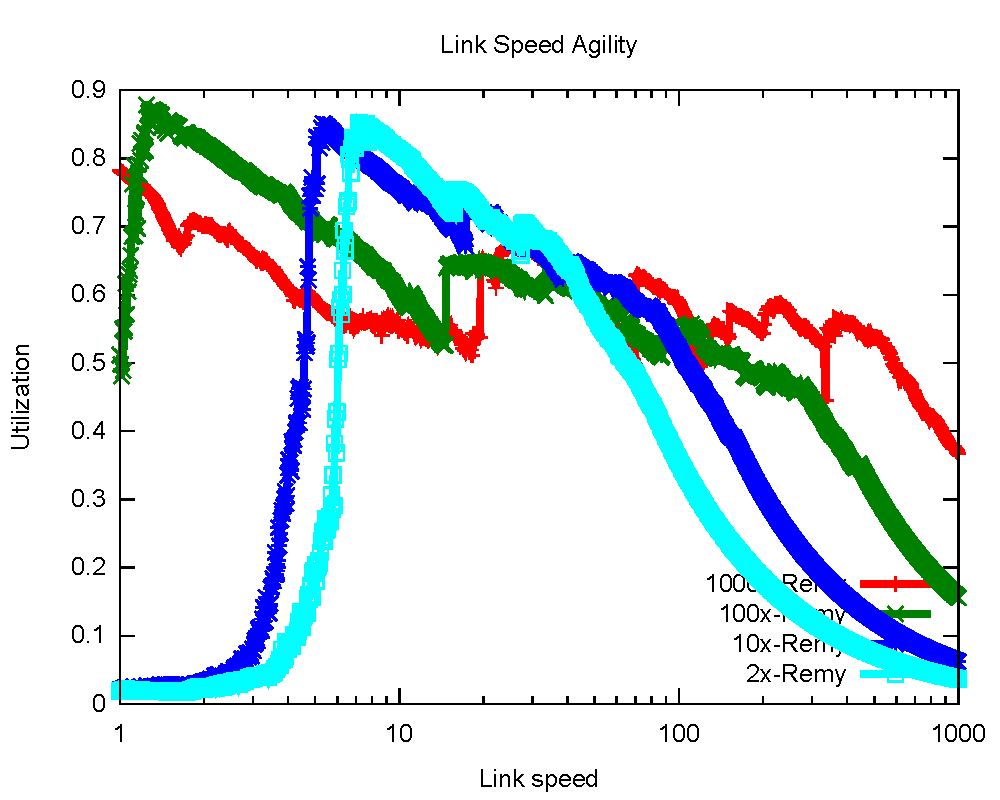
\includegraphics[width=\textwidth]{tradeoff-tpt.pdf}
%\end{subfigure}
%\begin{subfigure}[b]{0.33\textwidth}
%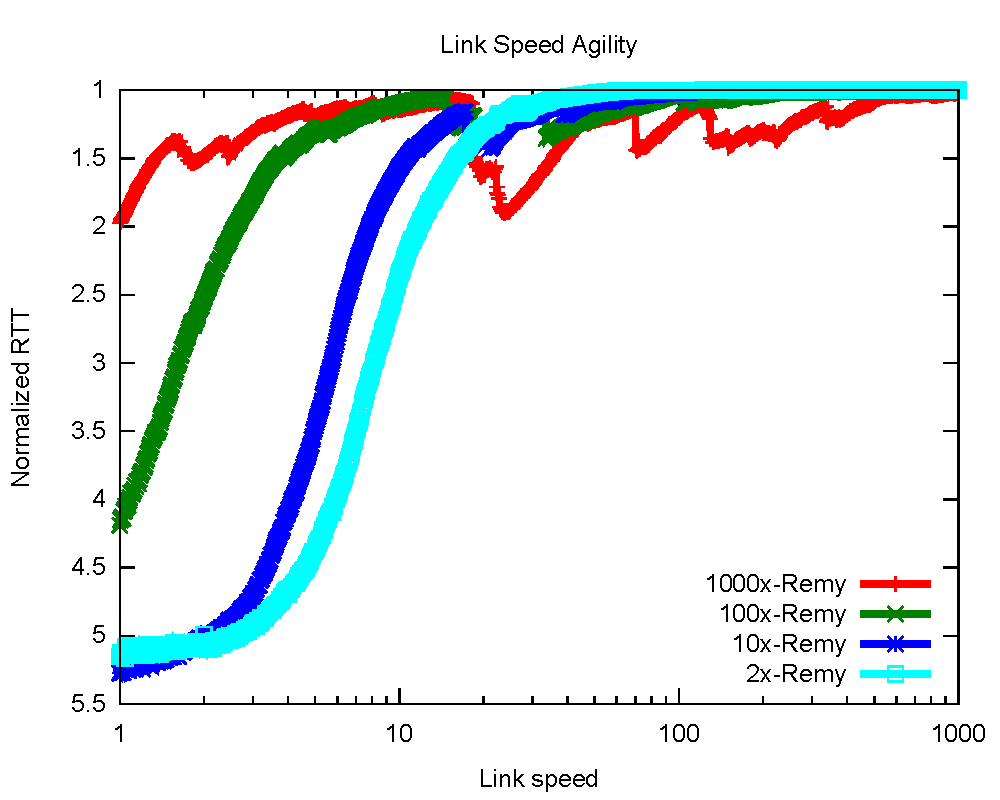
\includegraphics[width=\textwidth]{tradeoff-delay.pdf}
%\end{subfigure}
%\begin{subfigure}[b]{0.49\textwidth}
%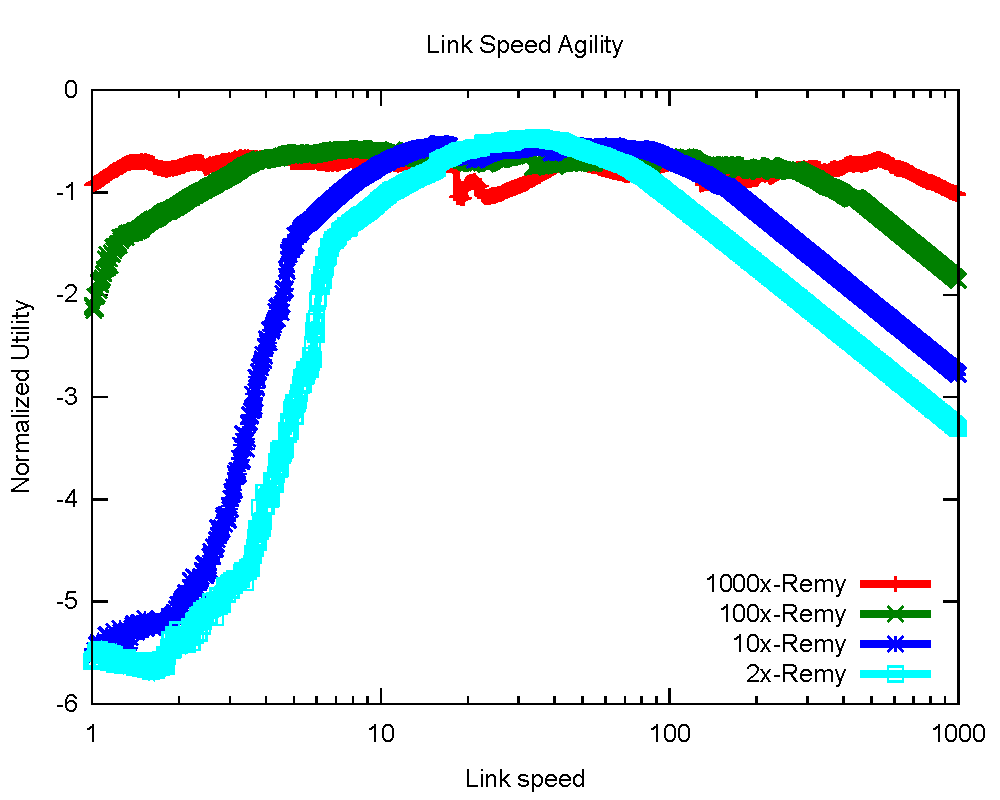
\includegraphics[width=\textwidth]{tradeoff-util.pdf}
%\end{subfigure}
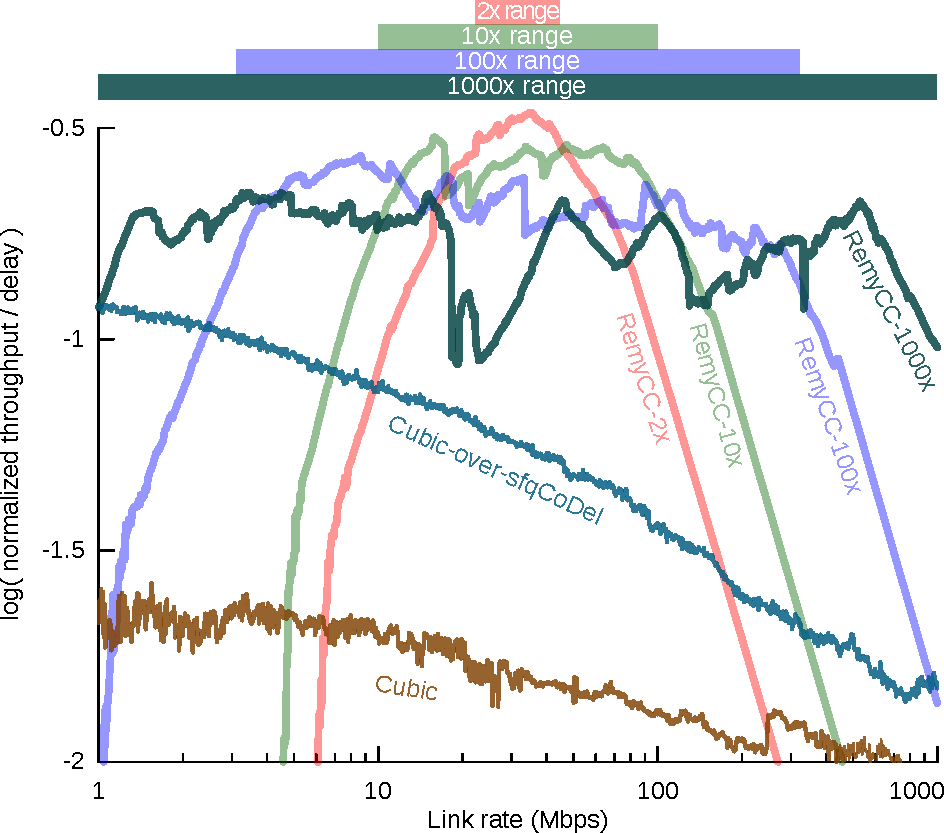
\includegraphics[width=\columnwidth]{oprange-manual.pdf}
\caption{Evidence of a weak tradeoff between operating range of a
  congestion-control protocol and performance. The RemyCC protocols
  designed with more specific network models (RemyCC-2x and RemyCC-10x)
  performed modestly better---within their design ranges---than protocols
  designed for a broader range of networks (RemyCC-100x and RemyCC-1000x),
  at a cost of deterioration when the actual network did not fall
  within the training scenarios. The four RemyCC protocols outperformed
  Cubic and Cubic-over-sfqCoDel over their respective design ranges.}
\label{fig:breadth}
\end{figure}

We find evidence of a weak tradeoff between operating range and
performance---optimizing for a smaller range did help modestly over
that range.  However, the improvements in objective from narrowing
down the operating range were modest, and each Tao (including the
Tao-1000x) outperformed existing algorithms over its full design
range.

\subsection{Structural knowledge}
\label{ss:topological}

\begin{figure}
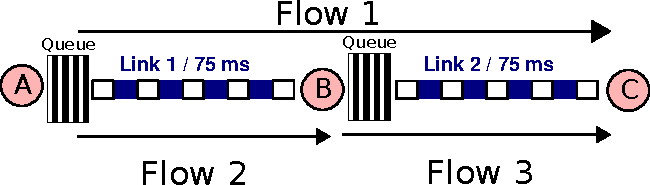
\includegraphics[width=\columnwidth]{twolink.pdf}
\caption{Parking-lot topology used to measure the consequences of imperfect
knowledge about the network's structure.}
\label{fig:two-link}
\end{figure}

We evaluated the difficulty of designing a congestion-control
protocol, subject to imperfect knowledge of the network's structure or
topology.

It is an understatement to say that the Internet is a vast network
whose full structure is known to nobody and which no model can
accurately capture. Nonetheless, researchers regularly develop new
distributed protocols for the Internet, which are deployed based on
tests in example network paths that imperfectly capture the Internet's
true complexity.

In practice, protocol designers expect that they can reason about the
performance of a distributed network algorithm by modeling the network
as something simpler than it is. We worked to capture that intuition
rigorously by studying quantitatively how difficult it is to learn a
congestion-control protocol for a more-complicated network, given a
simplified model of that network's structure.

In ns-2, we simulated a network with two bottlenecks in a
``parking-lot'' topology, shown in Figure~\ref{fig:two-link}. Flow 1
crosses both links and encounters both bottlenecks. It contends with
Flow 2 for access to the bottleneck queue and note A, and contends
with Flow 3 for access to the bottleneck queue at node B.

\begin{figure}[t!]
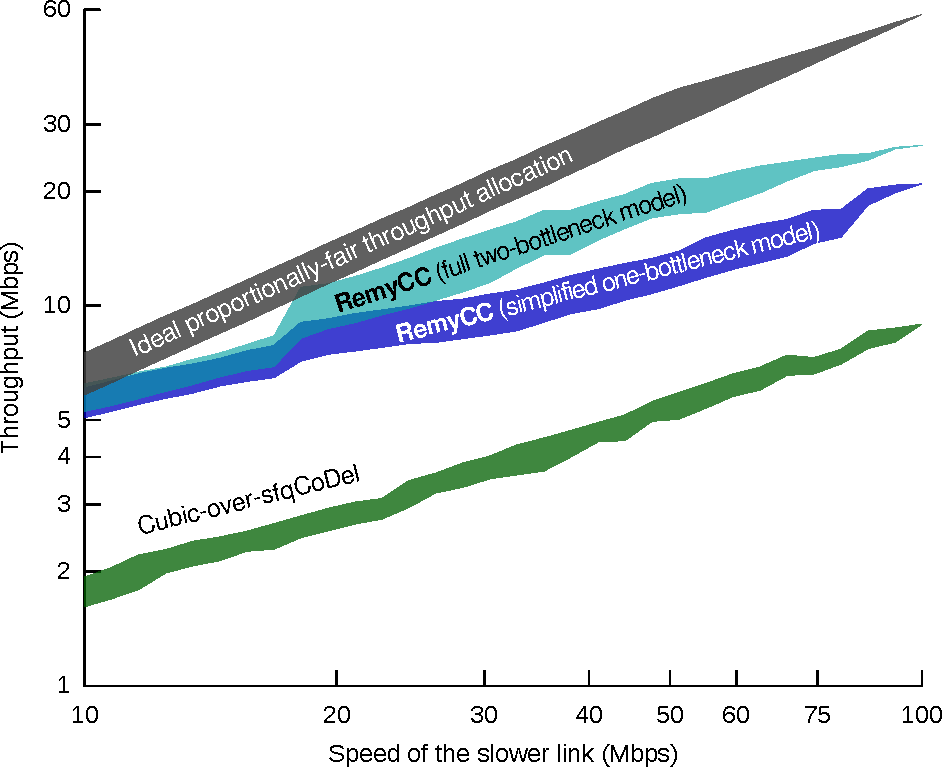
\includegraphics[width=\columnwidth]{multilink-all.pdf}
\caption{How well do endpoints need to understand the network around
  them? To assess this, we measure the throughput of four
  congestion-control schemes across a simulated two-hop network path,
  as the rate of each link is swept between 10 and 100~Mbps, with
  75~ms of delay per hop. A RemyCC designed for a simplified
  one-bottleneck model of the network performs 17\% worse, on average,
  than a RemyCC designed with knowledge of the network's true
  two-bottleneck structure. Both RemyCCs outperform TCP Cubic assisted
  by per-flow queueing and CoDel at the bottlenecks.}
\label{f:multihop}
\end{figure}

The results for Flow 1 (the flow that crosses both links) are shown in
Figure~\ref{f:multihop}.\footnote{Results for Flow 2 and Flow 3
  (flows crossing only a single link) were nearly identical between
  the schemes.} The experiment sweeps the rate of each of the two
links between 10 and 100~Mbps, and the shaded area in the figure shows
the full locus of throughputs seen by Flow 1. For each pair of rates
(for link 1 and link 2), we also calculate the ideal
proportionally-fair throughput allocation, and plot the locus of these
points as well.

Figure~\ref{f:multihop} shows the end-to-end throughput of connections
traversing two bottleneck links for different protocols, including two
RemyCCs. In each experiment, there were three flows: one that
traversed two hops (the measured connection), a cross-traffic flow
that traversed only the first bottleneck, and another cross-traffic
flow that traversed only the second bottleneck.

%of two Tao protocols, running over a simulated two-hop network path
%and contending with cross traffic that runs over the first or
%second link only.

As the rate of the first and second link are swept between 10 and 100
Mbps, the RemyCC that was designed for the actual network achieves
close to the ideal proportionally-fair throughput allocation across
the two links. This ideal serves as an upper bound on performance.

A RemyCC that was designed for a simplified model of the network with
only one hop also performs adequately, but a little worse than the
``full-complexity'' RemyCC. However, both computer-generated protocols
come closer to the ideal than contemporary protocols in wide use, TCP
Cubic~\cite{cubic}, the default TCP in Linux, running over per-flow
queueing and CoDel~\cite{CoDel}, an active queue management (AQM)
scheme that runs at both bottlenecks.

The results suggest that a congestion-control protocol designed for a
simplified model of the network's structure will experience a small,
but quantifiable, penalty to its performance.

\begin{table}
\centering
\begin{tabular}{l|l|l}
\bf Tao & \bf Links modeled & \bf Num.~senders \\
\hline
one-bottleneck & one, 150~ms delay & 2 \\
full-complexity & two, 75~ms delay each & 3 \\
\end{tabular}
\caption{Training scenarios used to measure the consequences of imperfect
  knowledge of the network structure. Both protocols were designed for
  link rates distributed log-uniformly between 10 and 100~Mbps, and
  for flows with mean ``on'' and ``off'' time of 1~second.
}
\label{table:topology-training}
\end{table}

\subsection{Knowledge about other endpoints}

\begin{figure*}[b!]
%\centering
%\begin{subfigure}[b]{\columnwidth}
%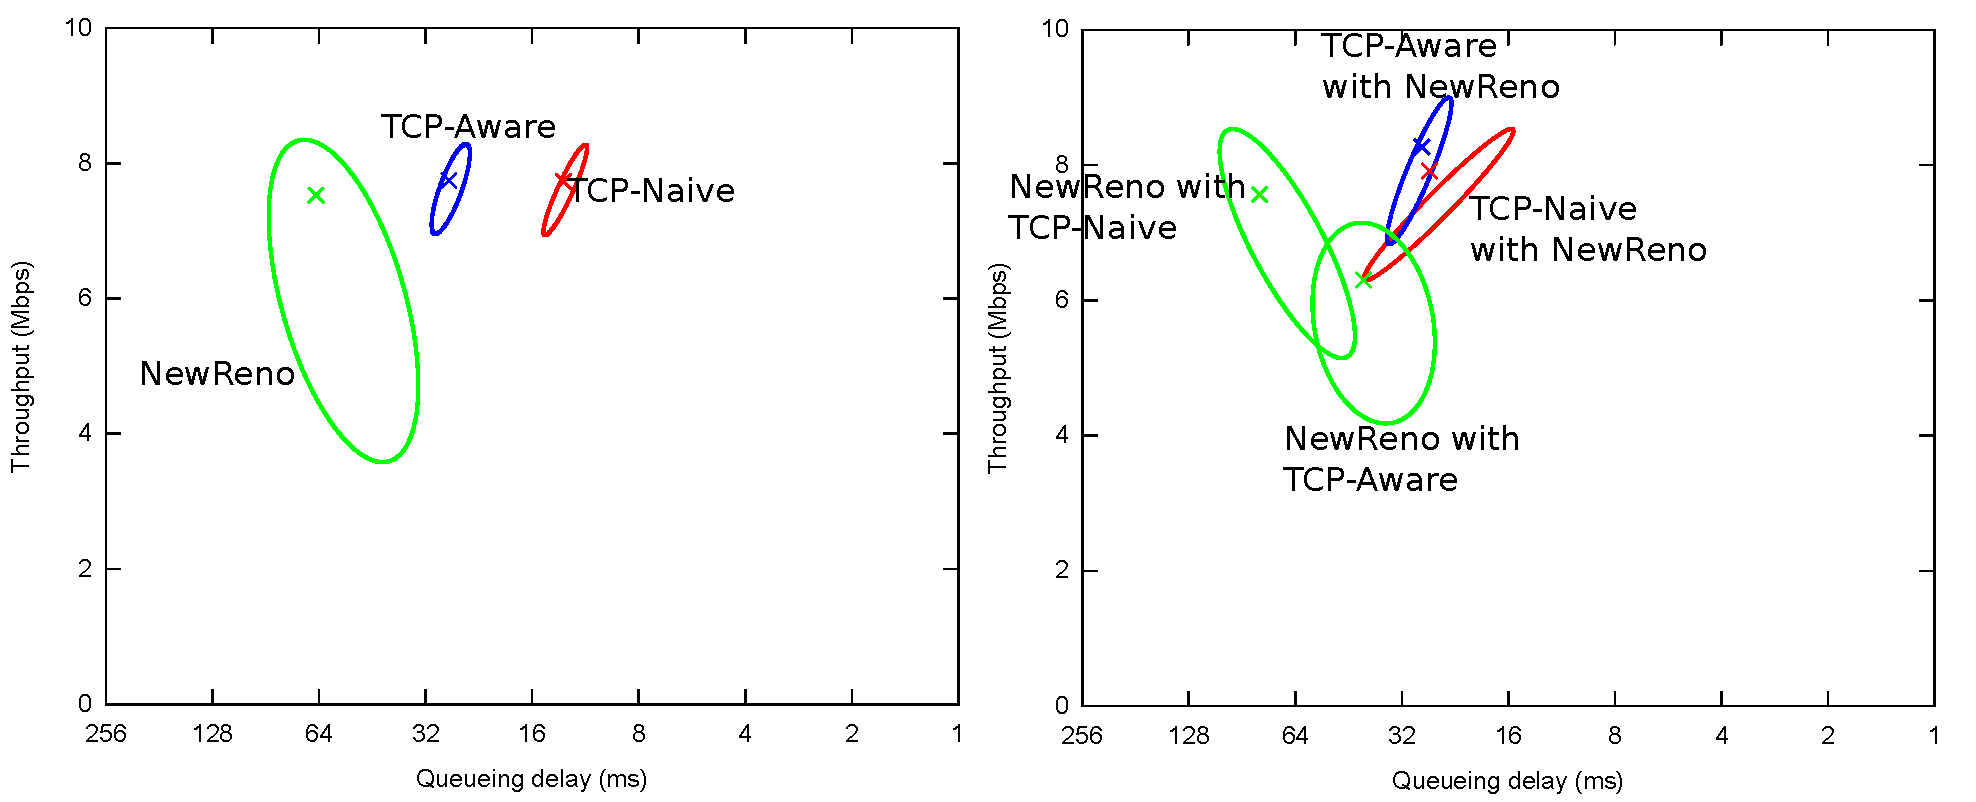
\includegraphics[width=\columnwidth]{compatible-5sec.pdf}
%\caption{TCP-Aware and TCP-Naive RemyCCs, 5 second ON/OFF}
%\end{subfigure}
%
%\begin{subfigure}[b]{\columnwidth}
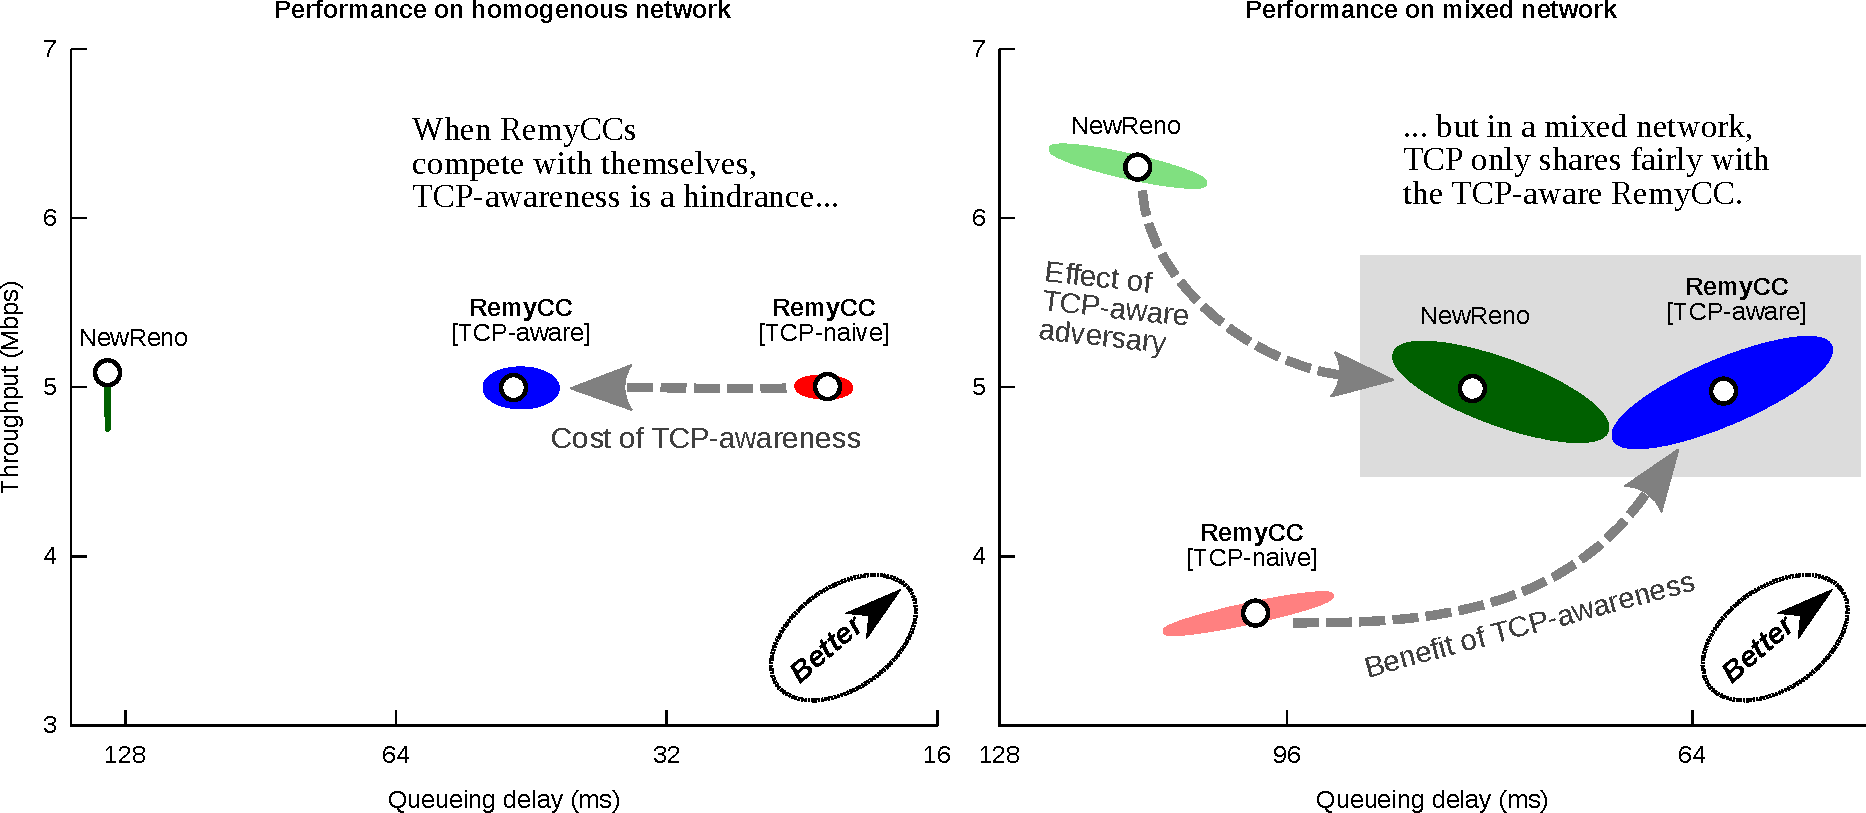
\includegraphics[width=\textwidth]{figures/manual/compatibility-drawn.pdf}
\caption{Tao protocols designed with and without TCP-awareness,
  competing against themselves or against TCP. Shown here, two
  endpoints contending for a 10~Mbps link with 100~ms RTT, 250 kB of
  buffer capacity (200~ms maximum queueing delay), and
  almost-continuous offered load. The fair share of throughput is
  5~Mbps per endpoint. Ellipses show 1-$\sigma$ range of results.}
%\end{subfigure}
\label{fig:tcpaware}
\end{figure*}

\label{s:tcpaware}

We investigated the consequences of designing a congestion-control
protocol with the knowledge that some cross-traffic may the product of
pre-existing incumbent protocols.

This question has considerable practical relevance; in practice, the
developer of a new network protocol will rarely be able to arrange a
``flag day'' when all endpoints switch to the new
protocol.\footnote{There has not been a ``flag day'' on the Internet
  since the switch to IP in 1983!}

On the broad Internet today, cross-traffic will typically be the
product of traditional loss-triggered TCP congestion-control
protocols, such as NewReno or Cubic. This status quo presents a
serious problem for new protocols that seek to perform differently or
that try to avoid building up standing queues inside the network.

Some protocols, such as Vegas~\cite{vegas}, perform well when
contending only against other flows of their own kind, but are
``squeezed out'' by the more-aggressive cross-traffic produced by
traditional TCP. Conventional wisdom is that any ``delay-based''
protocol will meet a similar fate. This has contributed to a lack of
adoption of Vegas and other delay-based protocols.

Ideally, a newly-designed protocol would perform well (e.g.~high
throughput, low delay) when interacting with other endpoints running
the same protocol, \textbf{and} would appropriately share a network
with incumbent endpoints running traditional TCP. But what are the
consequences of building this ``TCP-awareness'' into a protocol?

We studied this by designing two network protocols for a simple
network---one whose model specified that the cross-traffic would be
from the same protocol, and one whose model included a training
scenario where the cross-traffic was from traditional TCP half the
time.

The results are shown in Figure~\ref{fig:tcpaware}. In the left panel,
protocols compete only with cross-traffic from the same protocol. In
this homogeneous setting, adding TCP-awareness to a Tao protocol builds
up standing queues, more than doubling the queueing delay without
affecting throughput.

But in a mixed setting (Figure~\ref{fig:tcpaware}, right panel) where a Tao competes against TCP
NewReno, the TCP-naive Tao is squeezed out and does not get its fair
share of the link. In the shaded region showing the results when
NewReno competes with the TCP-aware Tao, TCP-awareness allows the Tao
to claim its fair share of the link and reduces the queueing delay
experienced both by itself and by TCP NewReno.

The results suggest that new delay-minded protocols \emph{can} avoid
being squeezed out by traditional loss-triggered TCP, but building in
this behavior comes at a cost to performance in the absence of TCP
cross-traffic.

\subsection{The relationship between different kinds of breadth}
\label{ss:parameter}

We report on the relationship between different kinds of breadth in a
protocol's training scenarios. We examined how a Tao protocol's design
breadth on \emph{one} axis---link rate---did or did not translate into
breadth when other axes varied, by testing it on a variety of
simulated networks.

These experiments bear on the question of what details about the network
a protocol designer must keep in mind when designing a protocol---is
it necessary to model a network's variation on every possible
characteristic, or it sufficient to model only variation in link speed
and a limited number of other characteristics that describe the
network?

As before, it would be preferable for a designer not to have to
model every axis on which the network might vary. If such simplifications
were permissible, that would suggest the problem of congestion control
was more easily learnable and designed protocols were more robust.

To do this, we use the Tao-1000x protocol designed earlier for a
thousand-fold range of link rates
(Table~\ref{table:oprange}). Although this protocol was designed with
only vague knowledge of the network's link rate, or in other words
with a broad design range of network link rates, it was designed with
very specific knowledge of the network's propagation delay (150~ms),
degree of multiplexing (two sender-receiver pairs contending for a
common bottleneck) and workload (a 50\% duty cycle for each
sender-receiver pair).

We have earlier found that the Tao-1000x protocol had excellent
``on-axis'' breadth (Figure~\ref{fig:breadth}) as the link rate itself
was varied, as it had been in the training scenarios.

By contrast, in this section we study the protocol's ``off-axis''
breadth---that is, how it performs on networks where we varied the
delay, cross-traffic workload, or degree of multiplexing outside the
model used to design the protocol. These testing scenarios are shown
in Table~\ref{table:p-learnability}.

\renewcommand{\columnwidth}{6 in}
\renewcommand{\textwidth}{6 in}

\begin{table}

\begin{subtable}{\columnwidth}
\small
\begin{tabular}{l|l|l|l|l|l}
\bf Link rate & \bf On avg. & \bf Off avg. & \bf min-RTT & \bf \#
senders & \bf buffer \\
\hline
33.2 Mbps & 1 sec & 1 sec & \cellcolor{blue!20} 10--300~ms & 2 & 5 BDP \\
\end{tabular}
\caption{Testing scenarios for measuring breadth in delay.}
\label{table:p-training}
\end{subtable}

\vspace{\baselineskip}

\begin{subtable}{\columnwidth}
\small
\begin{tabular}{l|l|l|l|l|l}
\bf Link rate & \bf On avg. & \bf Off avg. & \bf min-RTT & \bf \#
senders & \bf buffer \\
\hline
33.2 Mbps & 1 sec & \cellcolor{blue!20} 0.05--20~sec & 150~ms & 2 & 5 BDP \\
\end{tabular}
\caption{\ldots for measuring breadth in link rate.}
\end{subtable}

\vspace{\baselineskip}

\begin{subtable}{\columnwidth}
\small
\begin{tabular}{l|l|l|l|l|l}
\bf Link rate & \bf On avg. & \bf Off avg. & \bf min-RTT & \bf \#
senders & \bf buffer \\
\hline
33.2 Mbps & 1 sec & 1~sec & 150~ms & \cellcolor{blue!20} 1--20 & 5 BDP \\
\end{tabular}
\caption{\ldots for measuring breadth in the degree of multiplexing.}
\end{subtable}

\caption{Testing scenarios for relating a congestion-control
  protocol's designed breadth in one network characteristic (link rate)
  to its effective breadth in handling variation in other
  characteristics of the network.}
\label{table:p-learnability}

\end{table}

In each case, we plot the average throughput and delay achieved by the
Tao-1000x protocol. For reference, we compare this performance with
that of TCP Cubic and Cubic-over-sfqCoDel, which represent the current
widely-deployed status quo in end-to-end and in-network congestion
control.

We also plot the objective function---throughput divided by queueing
delay---as an all-around figure of merit for each protocol's
performance. As a rough guide, we consider cases where the Tao-1000x
protocol outperforms the status quo protocols to be acceptable
performance.

\begin{figure*}
\centering
\begin{subfigure}[b]{0.33\textwidth}
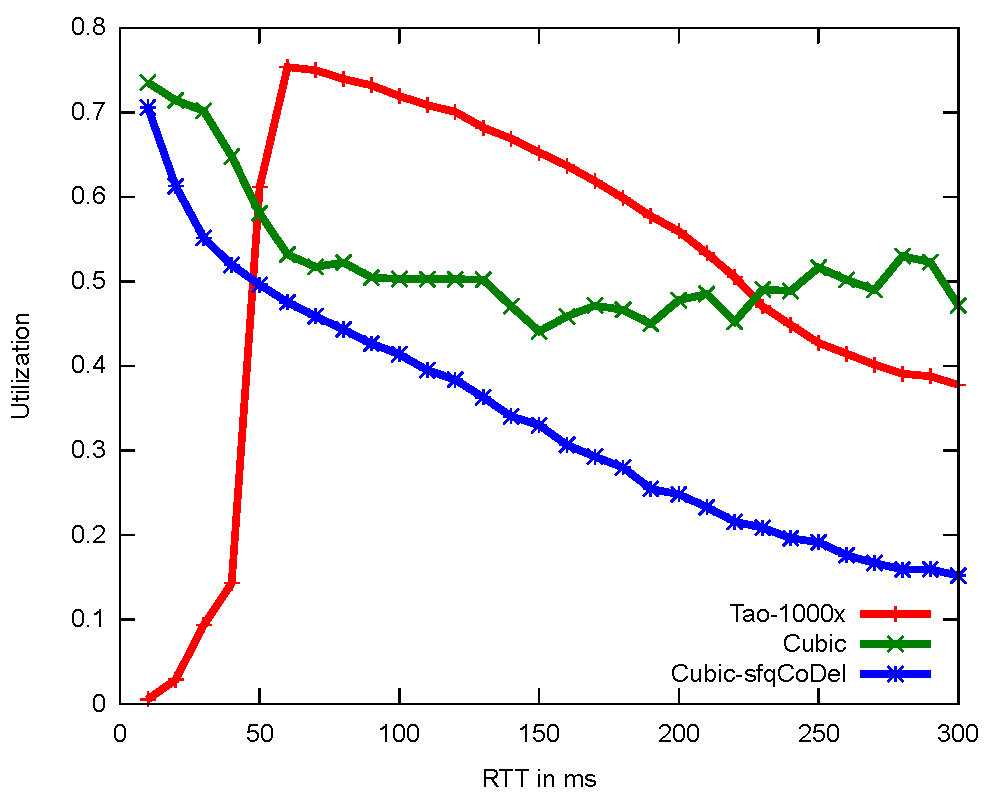
\includegraphics[width=\textwidth]{figures/rtt-agility-tpt.pdf}
\end{subfigure}
\begin{subfigure}[b]{0.33\textwidth}
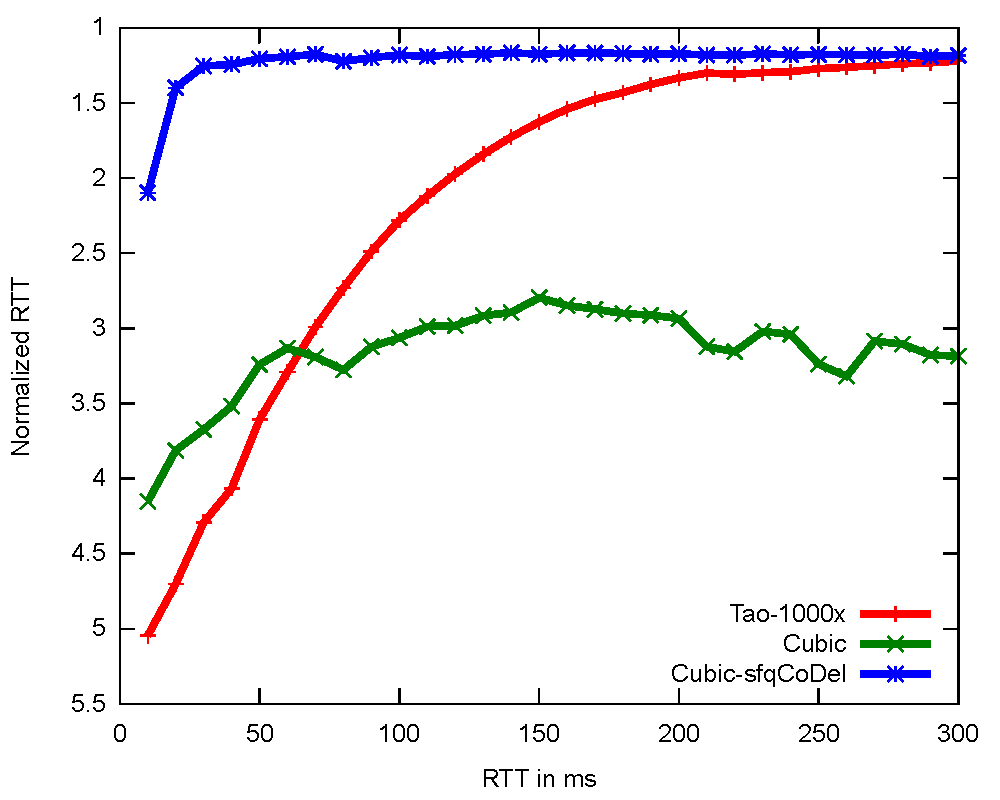
\includegraphics[width=\textwidth]{figures/rtt-agility-delay.pdf}
\end{subfigure}
\begin{subfigure}[b]{0.33\textwidth}
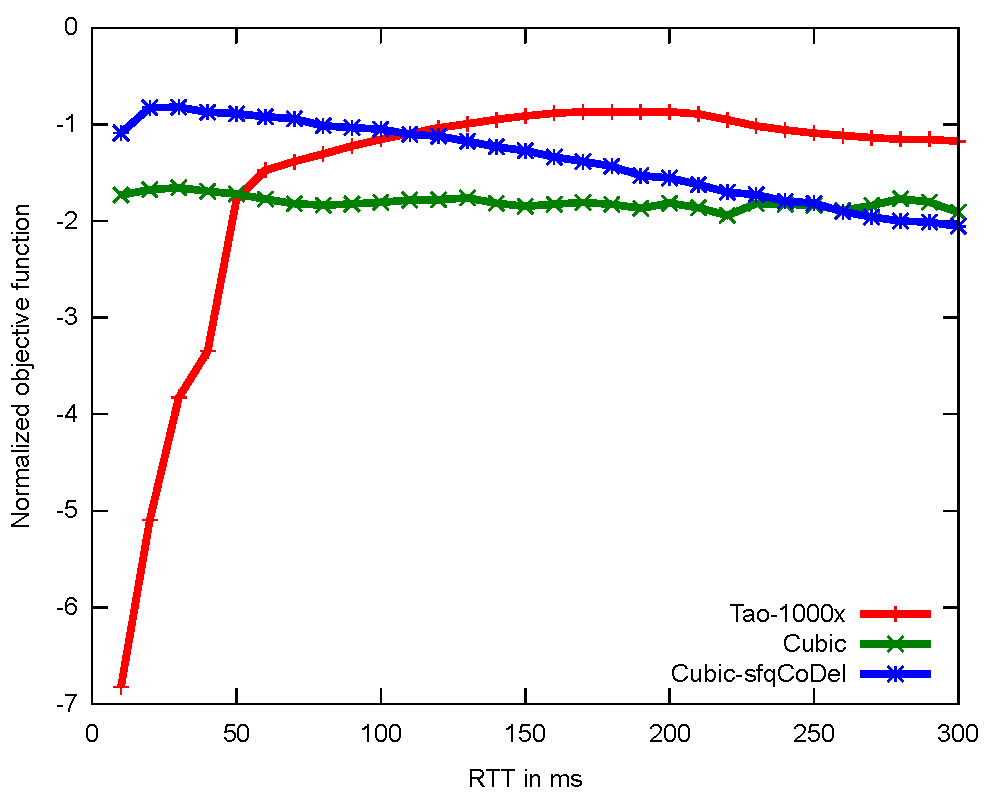
\includegraphics[width=\textwidth]{figures/rtt-agility-util.pdf}
\end{subfigure}
\caption{Off-axis performance as delay varied. The Tao-1000x protocol,
  designed for wide variation in link rate but an exact delay of
  150~ms, had good performance over delays above 50~ms, but suffered
  dramatically below that threshold.}
\label{fig:delay-agility}
\end{figure*}

\begin{figure*}
\centering
\begin{subfigure}[b]{0.33\textwidth}
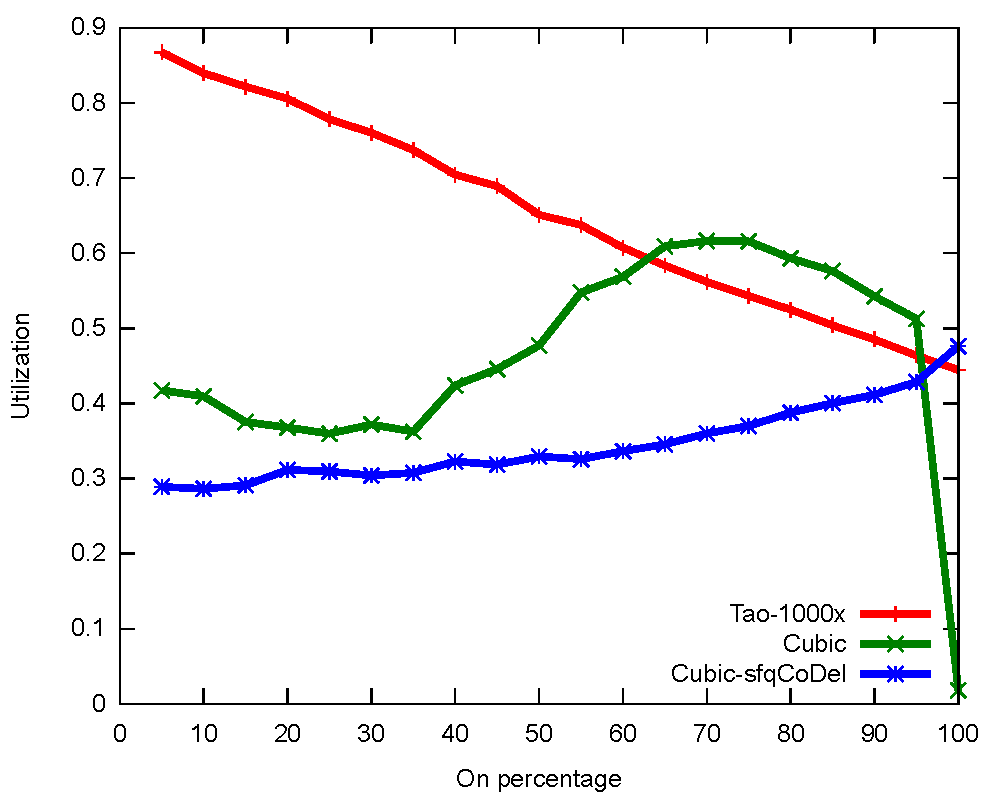
\includegraphics[width=\textwidth]{figures/workload-agility-tpt.pdf}
\end{subfigure}
\begin{subfigure}[b]{0.33\textwidth}
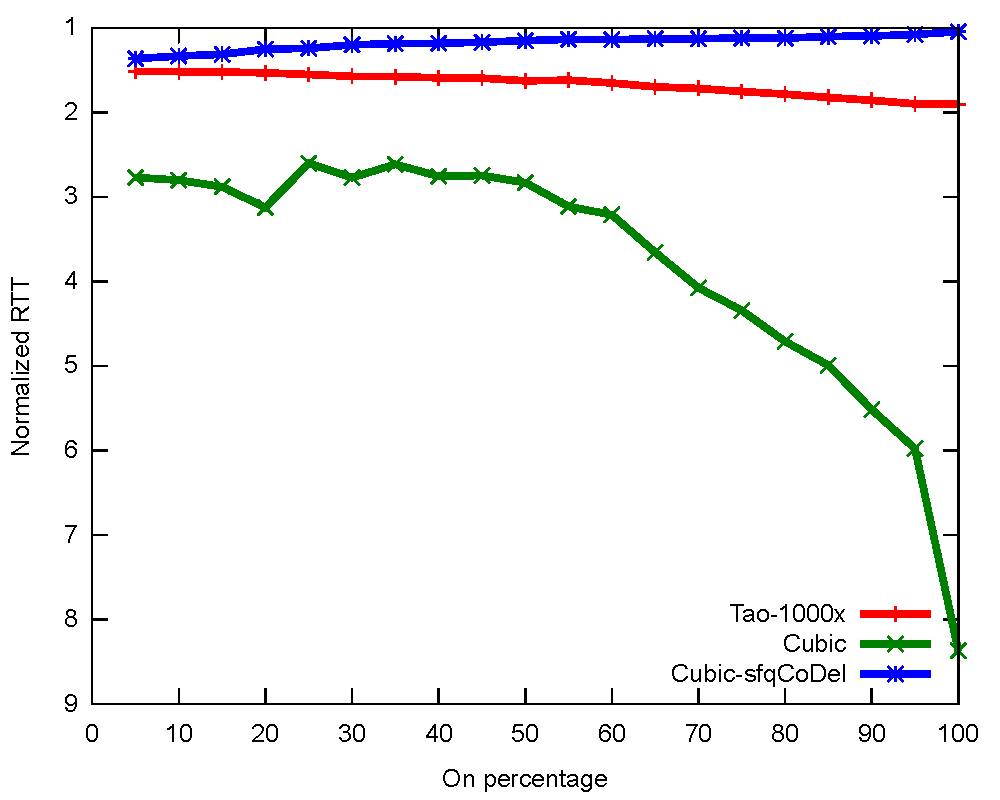
\includegraphics[width=\textwidth]{figures/workload-agility-delay.pdf}
\end{subfigure}
\begin{subfigure}[b]{0.33\textwidth}
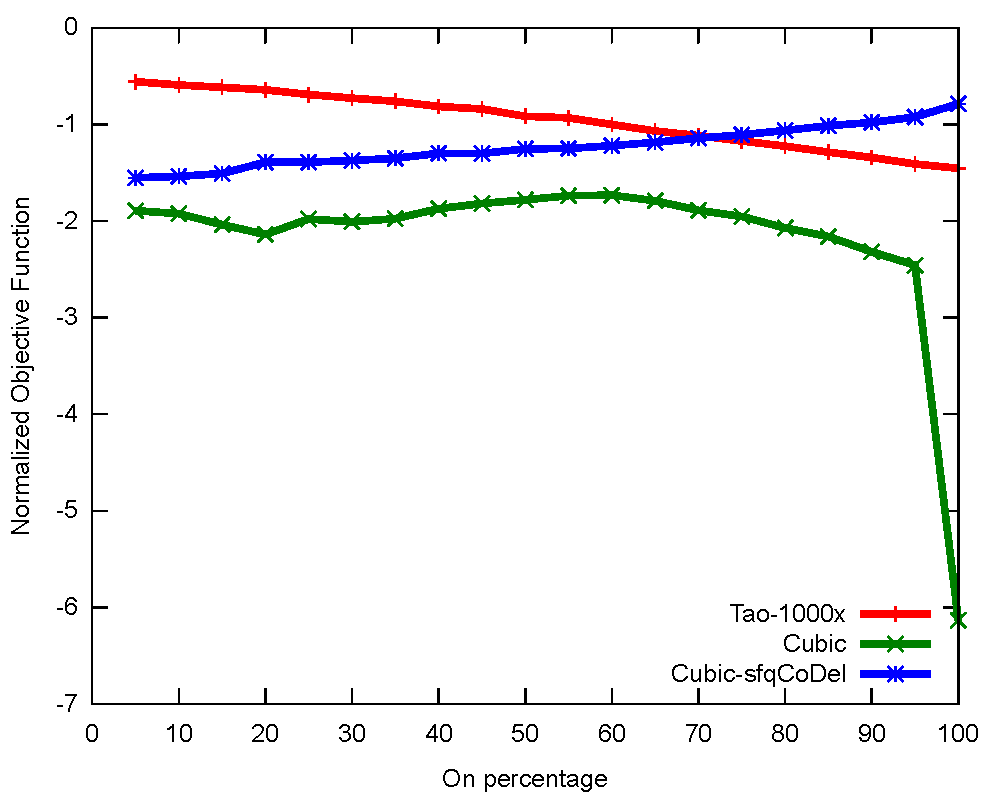
\includegraphics[width=\textwidth]{figures/workload-agility-util.pdf}
\end{subfigure}
\caption{Off-axis performance as workload varied. The Tao-1000x protocol,
  designed for wide variation in link rate but an exact cross-traffic
duty cycle of 50\%, performed well over a wide range of true duty cycles.}
\label{fig:workload-agility}
\end{figure*}

\begin{figure*}
\centering
\begin{subfigure}[b]{0.33\textwidth}
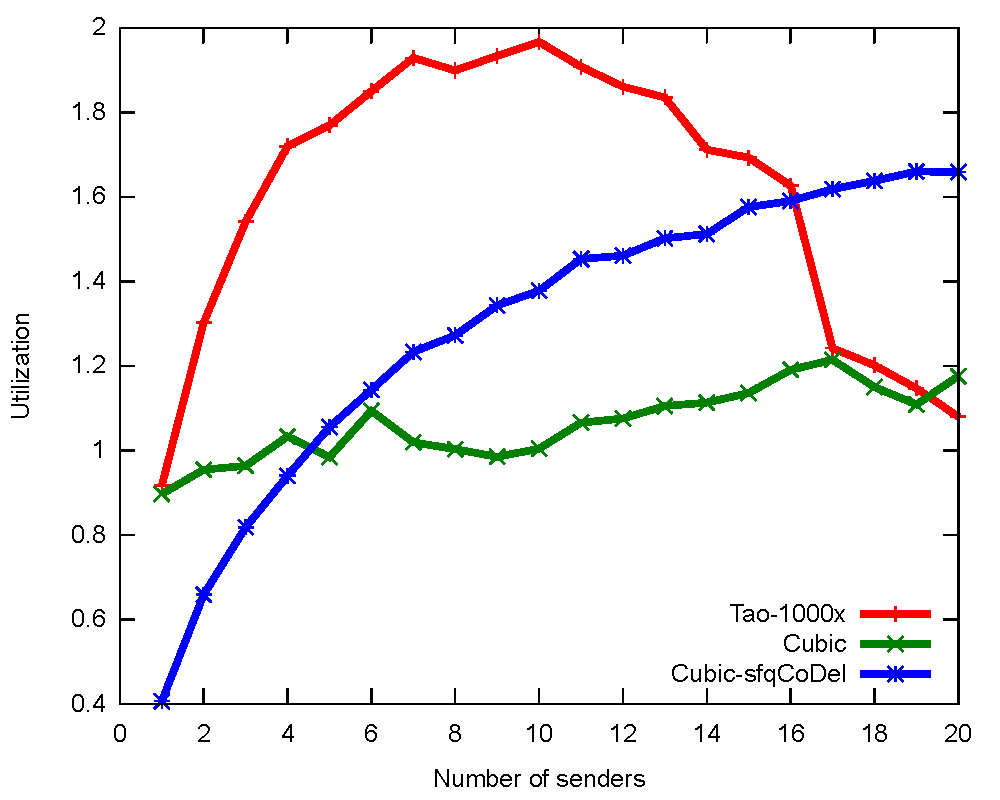
\includegraphics[width=\textwidth]{figures/muxing-agility-tpt.pdf}
\end{subfigure}
\begin{subfigure}[b]{0.33\textwidth}
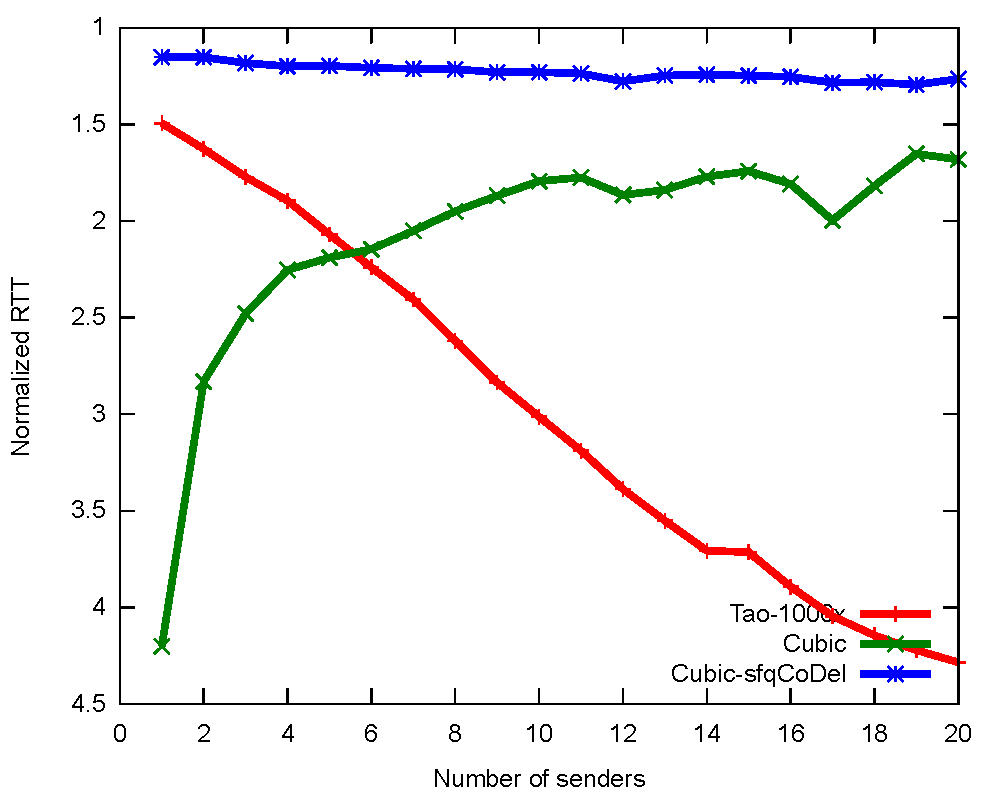
\includegraphics[width=\textwidth]{figures/muxing-agility-delay.pdf}
\end{subfigure}
\begin{subfigure}[b]{0.33\textwidth}
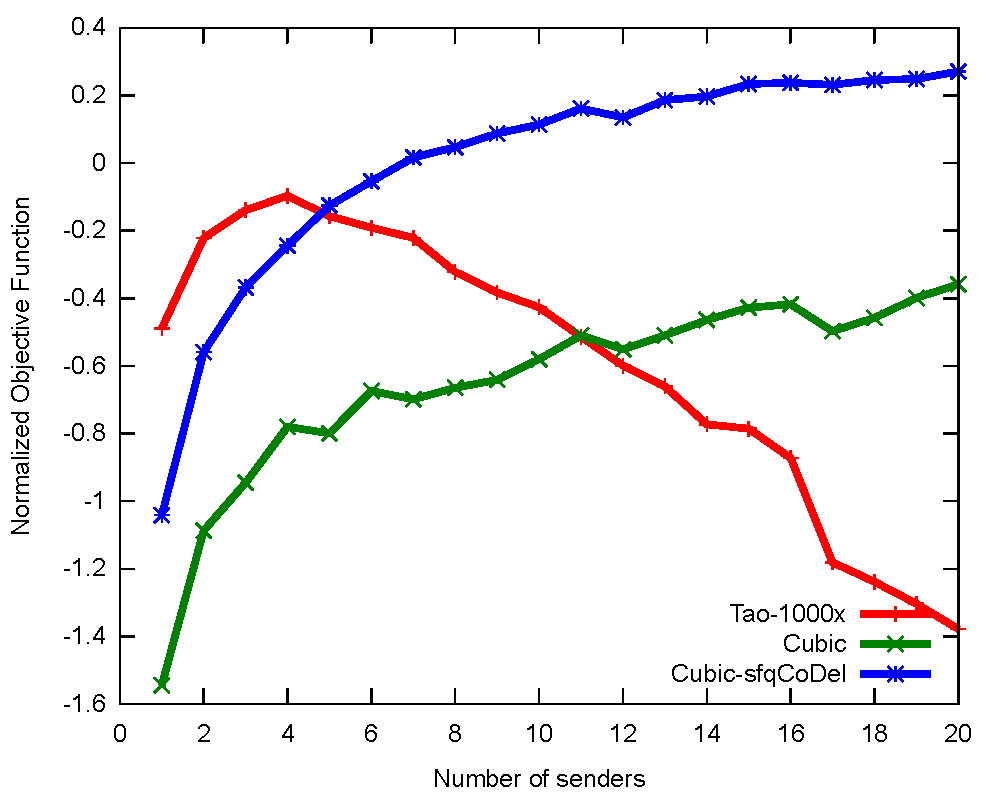
\includegraphics[width=\textwidth]{figures/muxing-agility-util.pdf}
\end{subfigure}
\caption{Off-axis performance as the degree of multiplexing
  varied. The Tao-1000x protocol, designed for variation in link rate but an
exact degree of multiplexing of two senders, performs worse than Cubic
as the true degree of multiplexing exceeds 10.}
\label{fig:multiplexing-agility}
\end{figure*}

We discuss each in turn below.

\subsection{Delay variation}

Recall that the Tao-1000x protocol was designed for an RTT of exactly
150~ms. In these experiments, we varied the minimum RTT between 5 and
300 milliseconds. The Tao protocol achieves better throughput and
delay compared with Cubic over the delay range between 50 and 300 ms,
and better throughput (at the expense of delay) compared with
Cubic-over-sfqCoDel.

Below 50 ms, the Tao protocol's performance falls off rapidly.  This
result suggests that breadth in link speed and delay are related but
not fully interchangeable.

To explore this relationship further, we designed Tao protocols with
differing amounts of breadth in the delay and link-rate axes
(Table~\ref{table:rtt-linkspeed}).

\begin{table}
\small
\begin{tabular}{l|l|l|l|l|l}
\bf Tao & \bf Link rates & \bf On avg. & \bf Off avg. & \bf min-RTT &
\bf \# senders \\
\hline
2x        & 22--44 Mbps & 1 sec & 1 sec & 150 ms & 2 \\
rtt+link  & 22--44 Mbps & 1 sec & 1 sec & 50--250 ms & 2 \\
rtt-10    & 33 Mbps & 1 sec & 1 sec & 110--200 ms & 2 \\
rtt-20    & 33 Mbps & 1 sec & 1 sec & 50--250 ms & 2 \\
rtt-30    & 33 Mbps & 1 sec & 1 sec & 10--280 ms & 2 \\
\end{tabular}
\caption{Tao protocols designed for breadth in delay.}
\label{table:rtt-linkspeed}
\end{table}

Figure~\ref{fig:rtt-robustness} shows the results: training
exclusively for variation in link speed creates a congestion-control
protocol whose objective tails off at lower RTTs. However, adding a
little variation in minimum RTT to the training scenario creates a
protocol that is \emph{almost} as good as a protocol trained exclusively for
variation in minimum RTT at that particular link speed.

\begin{figure*}
\centering
\begin{subfigure}[b]{0.33\textwidth}
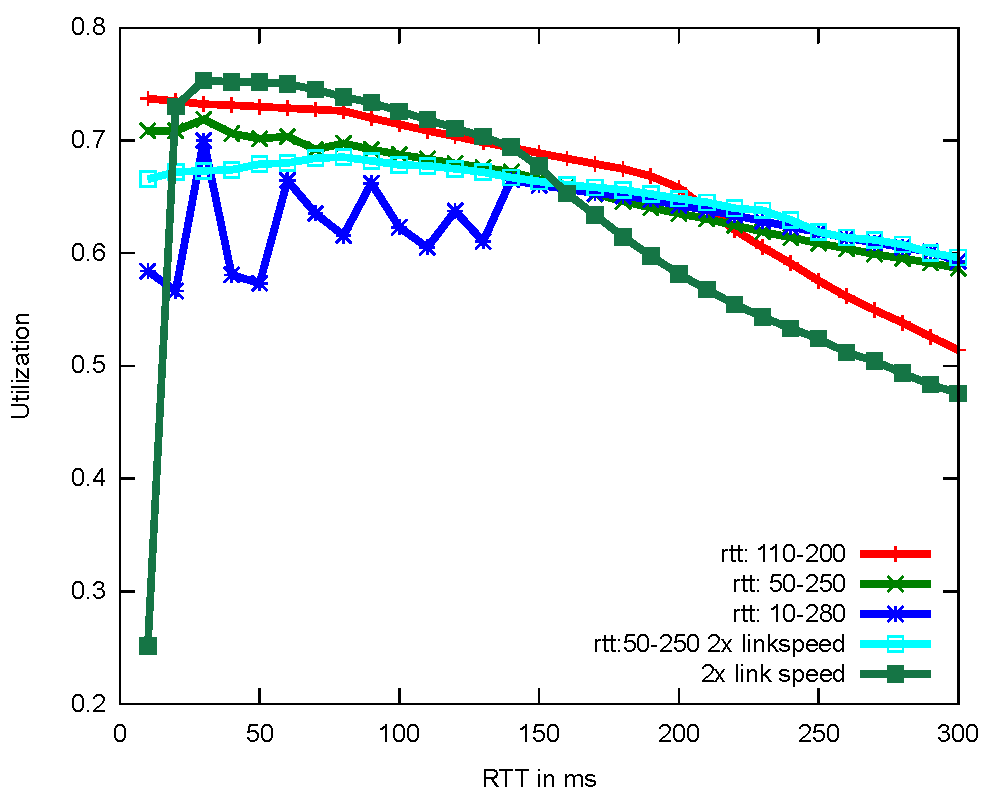
\includegraphics[width=\textwidth]{figures/rtt-robust-tpt.pdf}
\end{subfigure}
\begin{subfigure}[b]{0.33\textwidth}
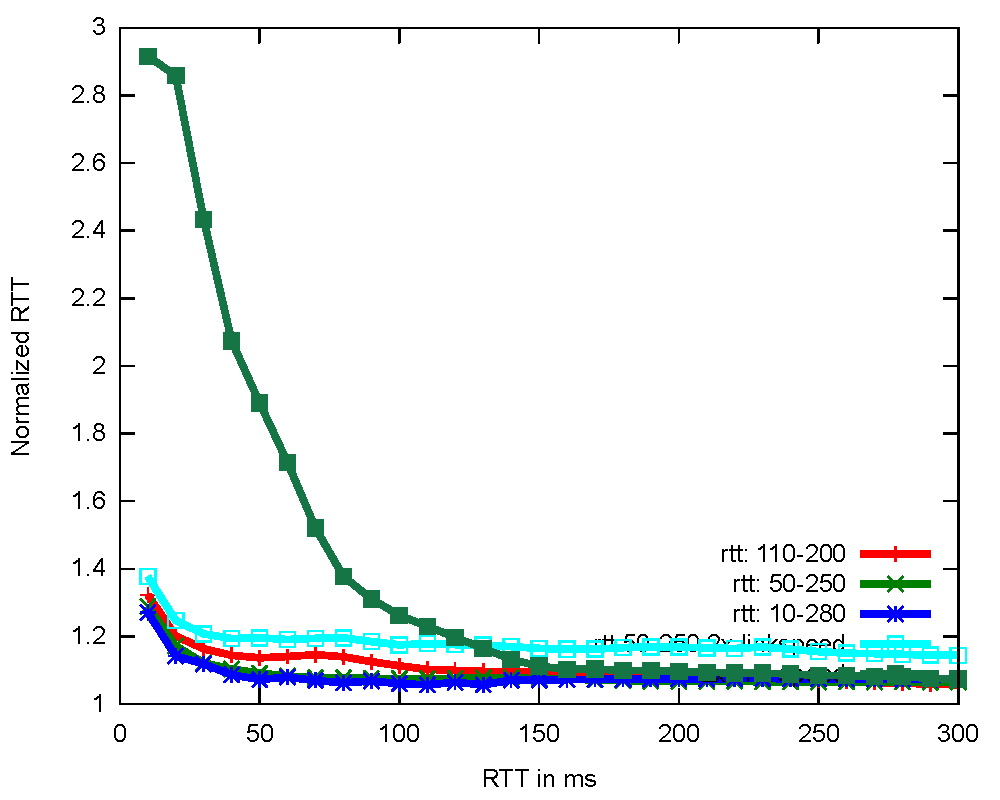
\includegraphics[width=\textwidth]{figures/rtt-robust-delay.pdf}
\end{subfigure}
\begin{subfigure}[b]{0.33\textwidth}
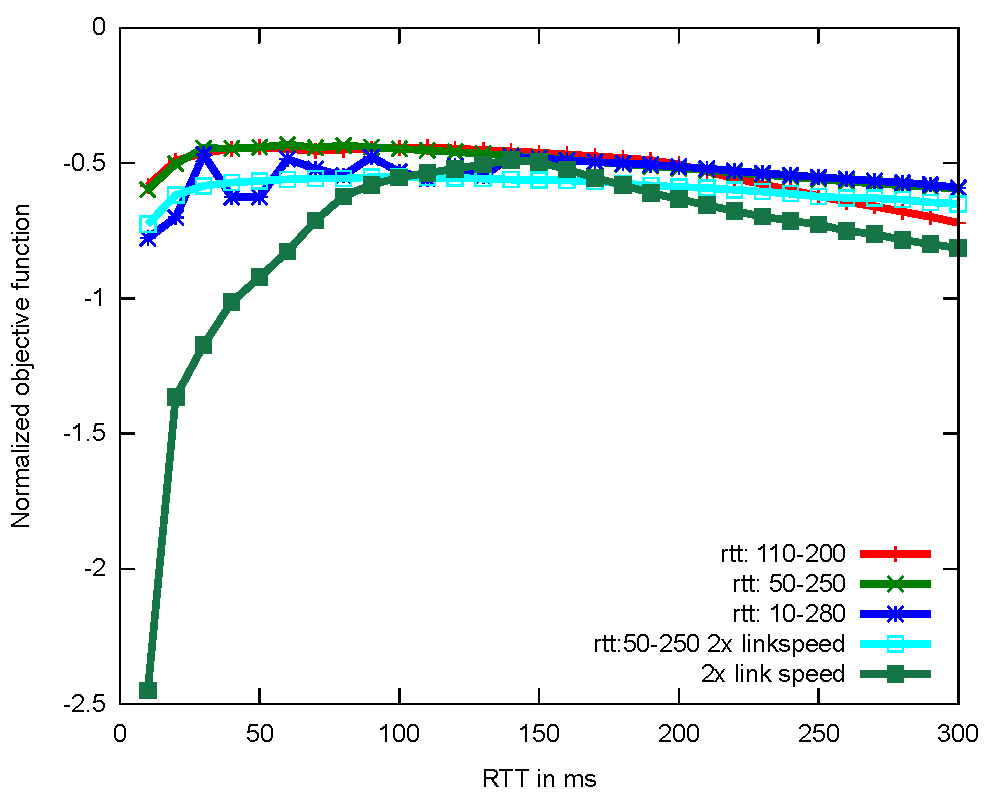
\includegraphics[width=\textwidth]{figures/rtt-robust-util.pdf}
\end{subfigure}
\caption{Breadth on the minimum RTT and link speed axis are related,
  but not fully interchangeable.}
\label{fig:rtt-robustness}
\end{figure*}

\begin{figure*}
\centering
\begin{subfigure}[b]{0.33\textwidth}
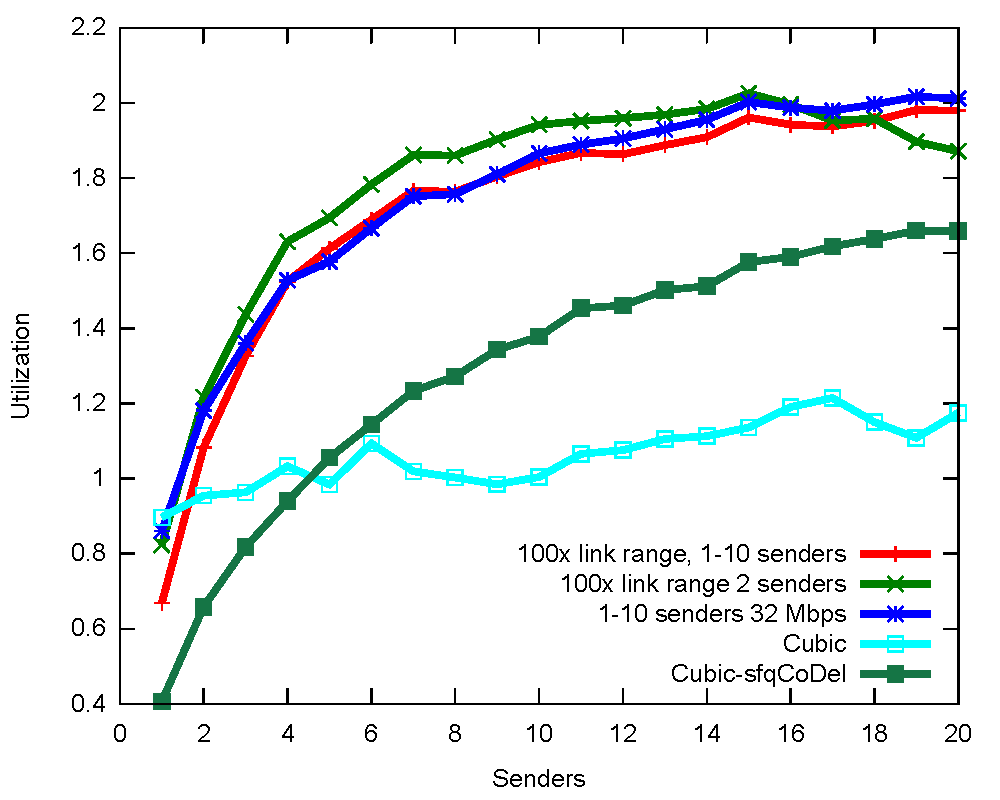
\includegraphics[width=\textwidth]{figures/muxing-robust-tpt.pdf}
\end{subfigure}
\begin{subfigure}[b]{0.33\textwidth}
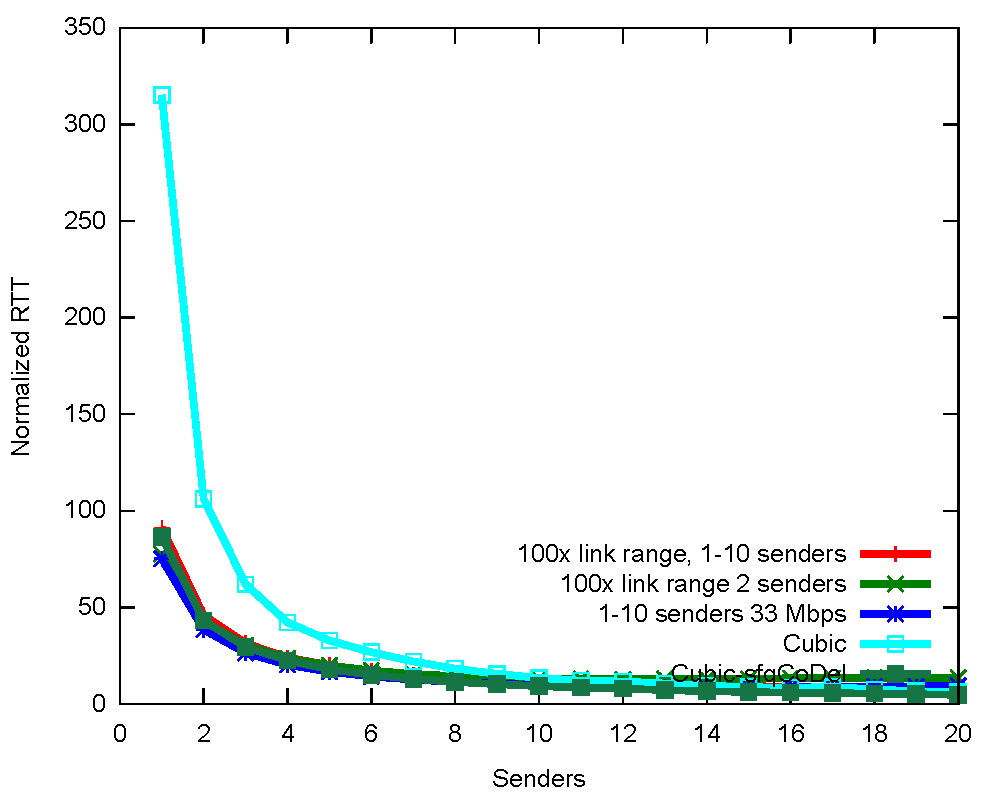
\includegraphics[width=\textwidth]{figures/muxing-robust-delay.pdf}
\end{subfigure}
\begin{subfigure}[b]{0.33\textwidth}
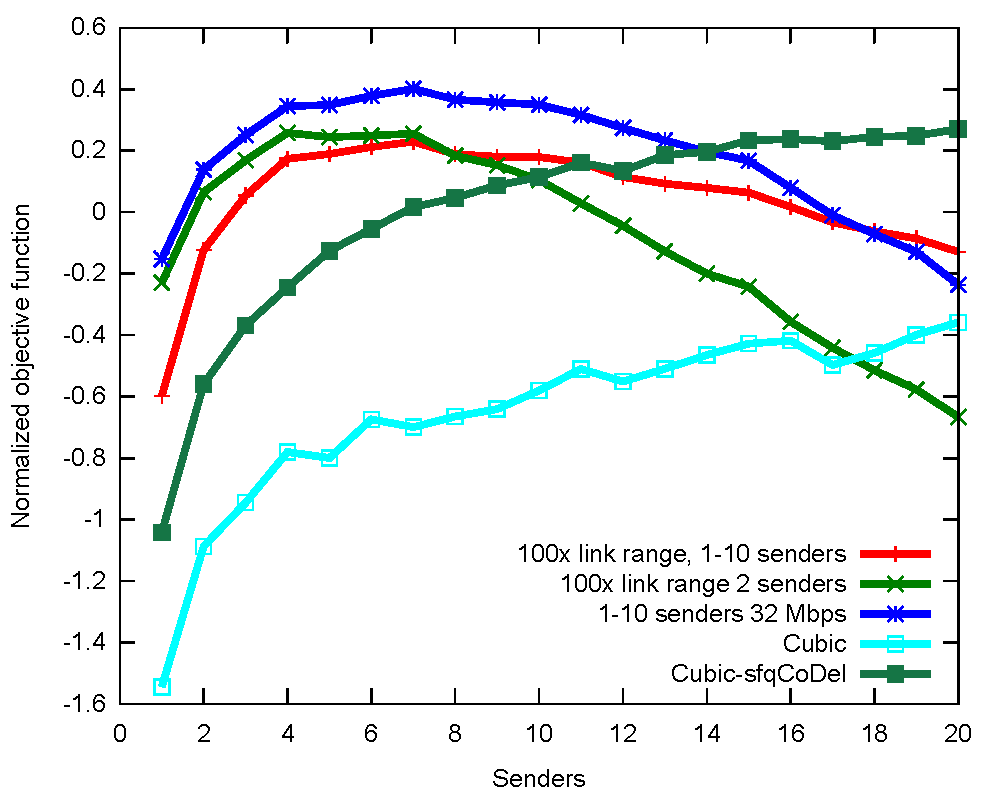
\includegraphics[width=\textwidth]{figures/muxing-robust-util.pdf}
\end{subfigure}
\caption{Learnability on the multiplexing and link speed axis are not interchangeable}
\label{fig:multiplex-robustness}
\end{figure*}

\subsection{Workload variation}

The Tao-1000x protocol was designed for an application whose offered load
kept the sender ``on'' for an average of 1~second, then ``off'' for a
pause time averaging 1~second between new offered load, producing a
duty cycle of 50\% for each of the two senders.

In these experiments, we varied the ``off'' time in order to explore
duty cycles between 5\% and 100\%.

Figure~\ref{fig:workload-agility} shows that the Tao protocol
outperformed Cubic on throughput and delay over almost the entire
range, and Cubic-over-sfqCoDel on throughput over the entire range. At
very high duty cycles, Cubic-over-sfqCoDel achieves higher
throughputs.

We looked at the behavior of the network in the time domain and found
that packet drops---which CoDel causes in order to control the
standing queues at the bottleneck---have only a mild effect on
performance if the queue always has pending data, as it does here when
both senders have a high duty cycle. This result has been
remarked-upon elsewhere~\cite{router-buffers}, where a higher offered
load\footnote{In that case, by increasing the number of senders}
permits a smaller buffer without compromising throughput.

At lower duty cycles, the Tao protocol profits (compared with Cubic)
by being able to quickly grab spare capacity on the link. Other
work~\cite{nwksleep, sprintip, linkoverload} has noted the benefits of
running networks at low utilization to be prepared for link
failures, a case where spare capacity is more likely to be had!

The results suggest that the workload presented by an application to a
congestion-control protocol need \emph{not} be closely modeled as part
of the protocol-design process.

\subsection{Multiplexing variation}

The Tao-1000x protocol was designed for a network with two sender-receiver
pairs exactly. In these experiments, we varied the maximum number of
concurrent flows between 1 and 20. The results are shown in
Figure~\ref{fig:multiplexing-agility}.

Before this experiment, we hypothesized that ``link rate per user''
might be a sufficient statistic for a distributed congestion-control
algorithm. If this hypothesis were true, a network with 10 users
contending for a 100~Mbps bottleneck link would be equivalent to a
network with 2 users contending for a 20~Mbps bottleneck link.

The results demonstrate that this hypothesis is not true. The Tao
protocol's breadth in link rate---even by a thousand-fold---did not
translate into commensurate breadth across different degrees of
multiplexing. This suggests that endpoints perceive the network's
degree of multiplexing, as an independent quantity from (and not
mediated through) their own fair share---meaning it is necessary to
model this quantity when designing a congestion-control protocol.

% TODO: Try and explain this if possible.

\subsection{Variation in all axes at the same time}

The previous experiments varied a single operating parameter at a
time. To evaluate the performance of the Tao-1000x protocol (designed for
link-speed variation only) across a broader range of operating
parameter combinations, we sampled 1000 random network configurations
with all four of these parameters (link rate, duty cycle, delay,
multiplexing) allowed to vary at once over broad ranges. The
distributions are shown Table~\ref{table:random-sampling}.

\begin{table}
\centering
\begin{tabular}{l|l|l|l}
\bf Link rate & \bf Duty cycle & \bf min-RTT & \bf \# senders \\
\hline
1--1000~Mbps & 5\--100\% & 50--300~ms & 1--100 \\
\end{tabular}
\caption{Testing scenario for all-axes variation experiment.}
\label{table:random-sampling}
\end{table}

To visualize our results, we plot the Tao protocol's performance
improvement relative to Cubic on the throughput and delay axis on an
indicator plot. As Figure~\ref{fig:random-cubic} shows, the protocol
generally outperforms Cubic on both throughput and delay. Compared
with Cubic-over-sfqCoDel (Figure~\ref{fig:random-cubicsfqCoDel}), the
Tao protocol does better on throughput at the cost of increased delay.

\begin{figure}
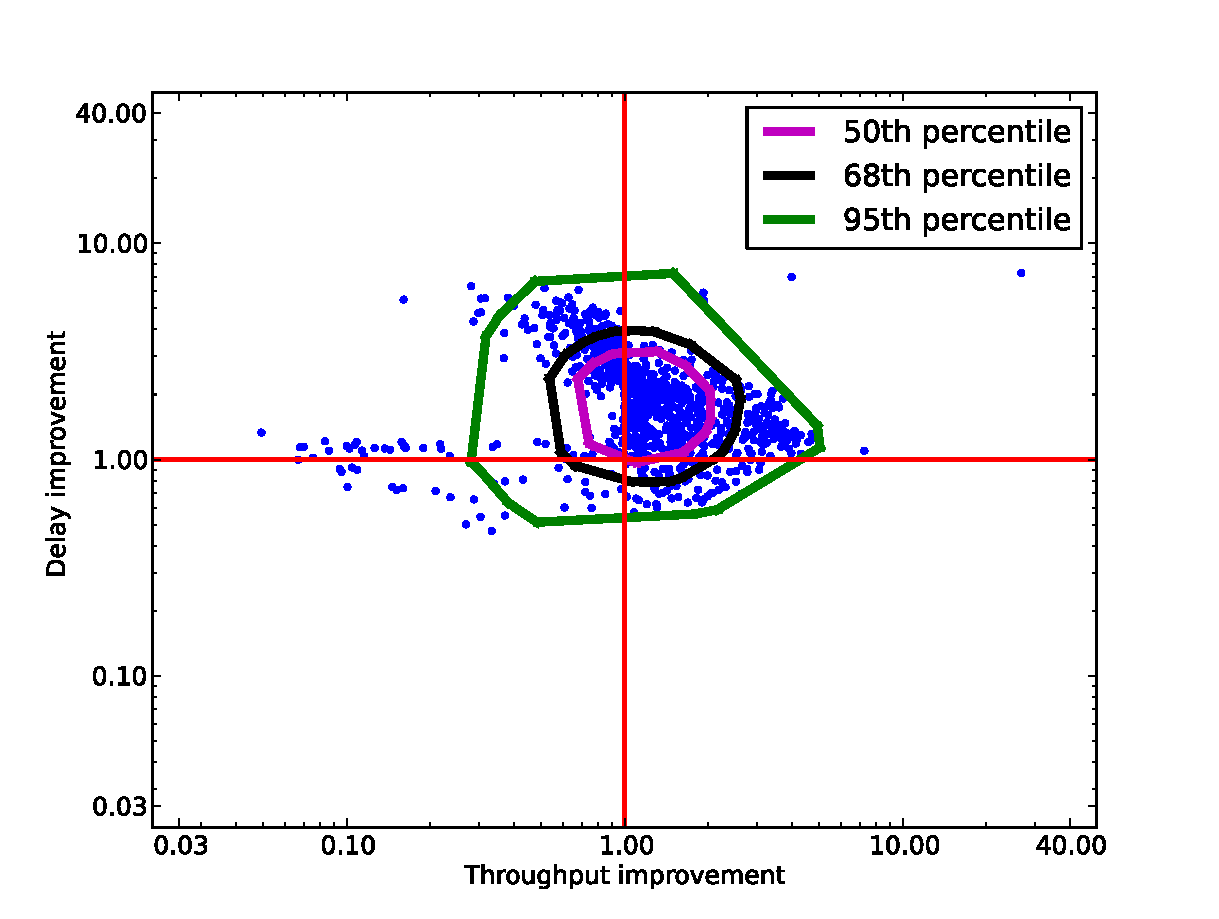
\includegraphics[width=\columnwidth]{cubic-10-empirical.pdf}
\caption{The Tao-1000x protocol, designed for breadth in link rate only,
  outperforms Cubic on most randomly sampled network configurations.}
\label{fig:random-cubic}
\end{figure}

\begin{figure}
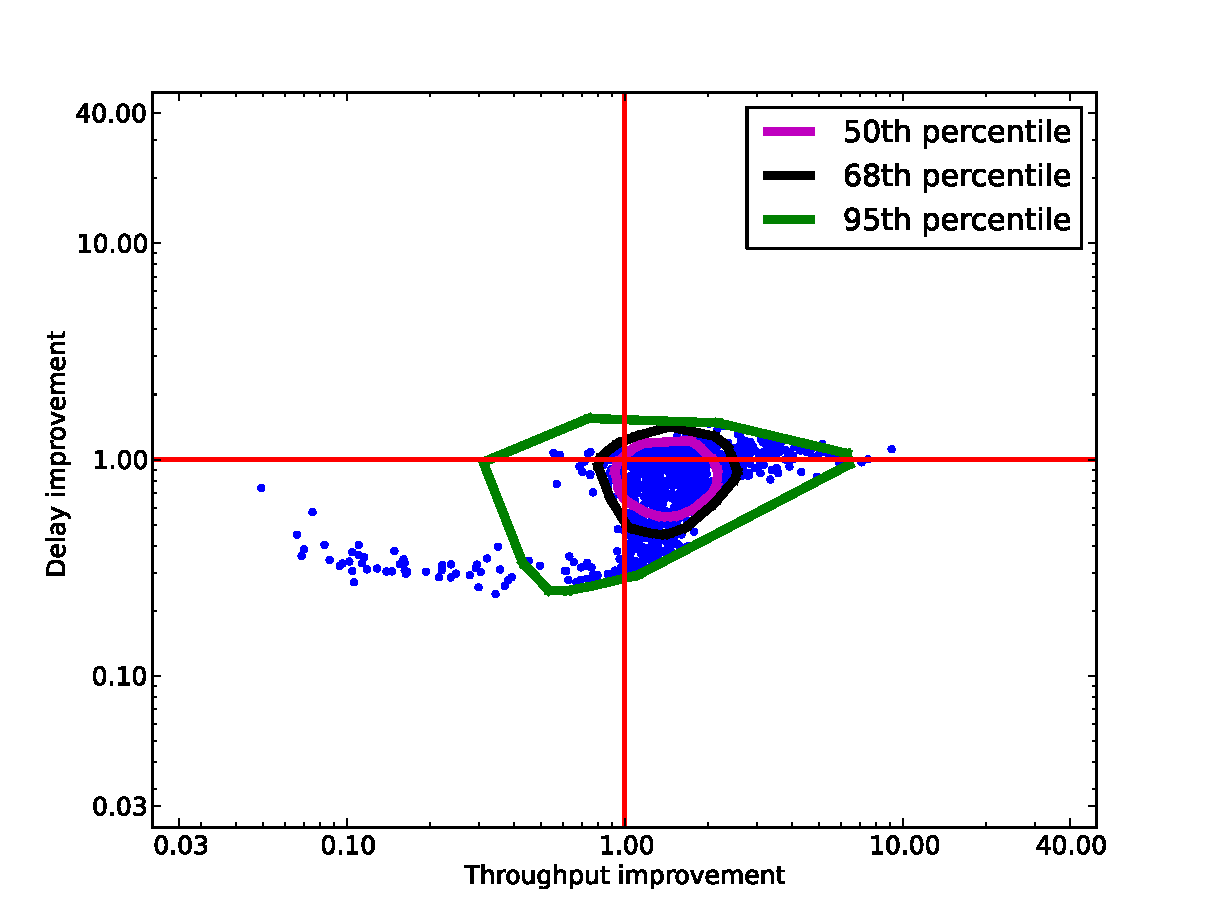
\includegraphics[width=\columnwidth]{cubicsfqCoDel-10-empirical.pdf}
\caption{The Tao-1000x protocol, designed for breadth in link rate only,
  achieves better throughput than Cubic-over-sfqCoDel, but at the
  expense of more delay}
\label{fig:random-cubicsfqCoDel}
\end{figure}
